\documentclass[fontsize=11pt, appendixprefix=true]{scrreprt}
\usepackage[magyar, english]{babel}                        % nyelvi csomag
\usepackage[T1]{fontenc}                                   % ékezetes betűknél is legyen automatikus elválasztás
\usepackage[utf8]{inputenc}                                % ékezetes betűk kezelése
\usepackage{lmodern}                                       % alapértelmezett betűtípus ne legyen pixeles
\usepackage{mathtools}                                     % képletekhez kell
\usepackage[style=ieee, backend=biber]{biblatex}           % bibliográfia
\usepackage{graphicx}                                      % képek beszúrása
\graphicspath{ {./images/} }
\usepackage[export]{adjustbox}                             % ez az ITK logó pozicionálásához kell
\usepackage[margin=2.5cm, bindingoffset=1.25cm]{geometry}  % margók
\usepackage[onehalfspacing]{setspace}                      % másfeles sorköz
\usepackage[hidelinks, unicode, pdfusetitle]{hyperref}     % kattintható tartalomjegyzék és hivatkozások
\usepackage{bookmark}                                      % PDF könyvjelzők
\usepackage{csquotes}                                      % a bibliográfiában megfelelően legyenek formázva az idézőjelek
%% \DeclareQuoteAlias{dutch}{magyar}

% Kódrészletekhez ajánlom
\usepackage{listings, scrhack}
\usepackage{sourcecodepro} % egy jó betűtípus
\lstset{captionpos=b, numberbychapter=false, basicstyle=\ttfamily, showstringspaces=false, columns=fullflexible}
%% \renewcommand\lstlistingname{kódrészlet}
\makeatletter
\renewcommand\fnum@lstlisting{\ifx\lst@@caption\@empty\else\thelstlisting.~\fi\lstlistingname}%
\makeatother

\titlehead{
  
\includegraphics[valign=m]{ITK_logo}
  \parbox[c]{\textwidth}{
    Pázmány Péter Catholic University\\
    Faculty of Information Technology and Bionics
  }
}

\subject{Thesis}
\addbibresource{bscthesis.bib}

\author{Dániel Balázs Becker\\Computer Science Engineering BSc}
\title{Abstracting Multimaterial Data Structures And Algorithms}
\date{2018}
\publishers{Supervisor:\\István Zoltán Reguly, PhD}

% Nyilatkozathoz két parancs definíciója
\newcommand{\pushtobottom}{\vspace*{\fill}}
\newcommand{\signatureline}[1]{\begin{flushright}
	\vspace*{.5cm}\par\noindent\makebox[2.5in]{\hrulefill}
	\par\noindent\makebox[2.5in][c]{#1}
	\end{flushright}
}

\begin{document}
\maketitle

\pushtobottom
I, undersigned Dániel Balázs Becker, student of the Faculty of
Information Technology and Bionics at Pázmány Péter Catholic University, declare
that I have written this thesis solely myself, without any unauthorized
help, and I have only used the sources referenced. Every part quoted word by
word or in a paraphrased manner is indicated clearly, with a reference made. I
have not submitted this thesis in any other training program.
\signatureline{Signature}

\tableofcontents
\newpage
\section*{Abstract}
Computations based on a structured or unstructured mesh, with the possibility of
accessing neighbouring elements, have wide-ranging applications in scientific
computing. Examples include fluid dynamics simulations, simulation of cellular
automata and the solution of partial differential equations (PDEs). As such,
there are innumerable implementations done by scientists and programmers both
for one-off experiments and for large software used in production. In many
cases, the computational performance achieved by such codes is vital for
scientific exploration, therefore many utilise modern many-core architectures
such as multi-core CPUs or GPUs.

Today's wide variety of modern many-core architectures, with their differing
programming styles, requires considerable programming effort to run applications
efficiently, making full use of the features and characteristics of the
available hardware. The programmer has to consider several levels of
parallelism; even CPUs now include wide vector units in each core, as well as
multiple cores, and various highly parallel hardware architectures such as GPUs
or FPGAs can be used either in addition to or instead of CPUs. The complex
memory hierarchies that often involve several levels of cache, which may be
explicitly programmable, present another difficulty as the programmer has to
take cache behaviour into account in order to make the code efficient.

If a certain piece of code needs to run well on multiple architectures, the
coding effort is multiplied, and subsequently maintenance is more difficult as
well --- any modification has to be applied to multiple codebases.

In my thesis we are working on an abstraction for describing such computations
at a high level, allowing fast experimentation and productivity. The abstraction
is designed in such a way that it can be automatically converted to various
high-performance implementations.

A critical feature of this abstraction is an extension to support a varying
number of materials, or species, at each grid point in the mesh, enabling much
more complex simulations. After examining real-world multimaterial computation
use cases, it becomes clear that devising a scheme that handles these
computations efficiently (both in terms of memory usage and speed) is
non-trivial. The main reason is that in most cases the vast majority of the mesh
cells only contain one material, which opens up the possibility for using more
economical (both in terms of memory and speed), compressed sparse data
structures to store the data.

In this work, we present the abstraction, which comes in the form of an Embedded
Domain Specific Language (eDSL) or ``active library'', the host language being
C++. This means that the framework can be used as if it were a traditional
software library and can be compiled with normal compilers, but the intended
usage for production applications is to use source-to-source compilation,
generating code specifically to take advantage of the target hardware
architecture. We also present examples of the most important computational
patterns implemented in our framework, both single material and multimaterial
cases.

\newpage
\section*{Kivonat}
\begin{otherlanguage}{magyar}
A strukturált és nemstrukturált térhálókon értelmezett, szomszédos elemek
elérését lehetővé tevő számítási minták nagyon gyakoriak a tudományos célú
számítógépes szimulációkban, többek között fluidikai szimulációk, celluláris
automaták szimulációja és parciális differenciálegyenletek megoldása
esetén. Ennek következtében mind kutatók, mind programozók számtalan
implementációt készítettek az ilyen típusú számítások elvégzésére, mind egyszeri
kísérletek céljából, mind nagyobb, tartós használatra készült programok
részeként. A programok számítási teljesítménye nagy jelentőséggel bír a
tudományos kutatásban való és egyéb felhasználás során, ezért sok implementáció
használ modern, többmagos architektúrákat, például többmagos CPU-kat és GPU-kat.

A ma elérhető modern, többmagos architektúrák sokfélesége jelentős programozói
erőfeszítést tesz szükségessé, mivel a különböző hardvereket különböző módokon
kell programozni, kiváltképp, ha a program hatékonyságának növelése érdekében az
eszköz tulajdonságait a lehető legnagyobb mértékben ki szeretnénk használni. A
párhuzamosságnak több szintjére kell odafigyelni: a modern CPU-k mindegyik magja
tartalmaz vektorizációs egységeket, a processzorok több magból állnak, és a
CPU-k helyett vagy mellett használhatunk nagyfokú párhuzamosságra képes
eszközöket is, például GPU-kat vagy FPGA-kat. A komplex, hierarchikus
memóriaarchitektúrák, amelyek több, akár explicite programozható cache-szintet
tartalmaznak, egy újabb nehézséget jelentenek a programozó számára, mivel
figyelembe kell vennie a cache sajátosságait ahhoz, hogy hatékony, a memóriát
jól használó programot írjon.

Ha egy adott kódnak többféle architektúrán kell hatékonyan futnia, a szükséges
programozási munka mennyisége is megsokszorozódik, és ennek következtében a
kódbázis karbantartása is sokkal nehezebbé válik, mivel minden változtatást több
helyen is végre kell hajtani.

A szakdolgozatom kapcsán egy olyan absztrakció létrehozásán dolgozunk, amivel a
fent leírt számítási minták könnyen, magas szinten leírhatók, lehetővé téve a
produktív, gyors kísérletezést. Az absztrakciót olyan módon terveztük meg, hogy
lehetőség legyen belőle különböző hardverarchitektúrákra optimalizált kódot
generálni automatikusan.

Az absztrakció egyik legjelentősebb eleme, hogy a térháló minden pontjában
egyszerre több anyag is jelen lehet, amivel sokkal komplexebb szimulációk
futtatása válik lehetségessé. A már létező több anyagos szimulációk vizsgálata
során egyértelművé vált, hogy egy olyan absztrakció kidolgozása, amely az ilyen
számításokat mind memóriahasználat, mind futási sebesség szempontjából
hatékonyan tudja elvégezni, nem triviális. Ennek oka az, hogy a legtöbb
szimulációban a cellák túlnyomó többsége mindössze egy anyagot tartalmaz, ezért
lehetőség nyílik a memóriahasználat és a futásidő tekintetében is gazdaságosabb,
tömörített ritka adatstruktúrák használatára.

Ezen szakdolgozatban bemutatjuk a megtervezett absztrakciót, amit egy a C++
programozási nyelvbe beágyazott domain-specifikus nyelv (eDSL) formájában
valósítunk meg. Ez azt jelenti, hogy a keretrendszer használható hagyományos
szoftverkönyvtárként, és a megírt kód lefordítható hagyományos C++ fordítókkal
is, de alapvetően a cél az egyes architektúrák sajátosságait hatékonyan
kihasználó kód automatikus generálása minden támogatott hardverarchitektúrára.
Az absztrakció ismertetése után bemutatjuk a legfontosabb számítási minták
implementációját a leírt absztrakció segítségével, mind egy anyagos, mind több
anyagos példákkal illusztrálva az keretrendszer használatának lehetőségeit.
\end{otherlanguage}

\chapter{Introduction}

In computational simulations in various scientific fields, the class of problems
that can be addressed by a model containing a spatial mesh, with data defined on
its cells and possibly also its edges, has proven to be very useful. Examples of
its use cases include computational fluid dynamics (CFD), computational
electro-magnetics (CEM), the simulation of cellular automata as well as the
solution of partial differential equations (PDEs).

In this chapter, we give a description of the challenges faced by programmers or
scientists who aim to make use of this computational model while trying to
utilise the full potential of the vast array of modern, parallel hardware
architectures available today. We describe how a high level abstraction can help
to overcome these difficulties without undue compromises in performance. We also
give an overview of existing approaches to this problem, and show in what ways
our proposed abstraction differs from these or extends them.

\section{Description of the problem}

\subsection{Structured vs. unstructured meshes}
\begin{figure}
    \centering
    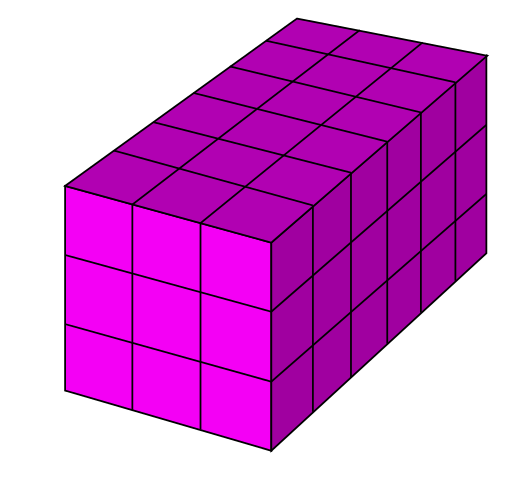
\includegraphics[width=0.25\textwidth]{structured_mesh}
    \caption{Structured Cartesian grid in 3D}
    \label{fig:structured_mesh}

    \small Source: By Mysid, Slffea - Drawn in CorelDraw by Mysid, based on a %
    JPEG by Slffea., CC BY-SA 3.0 %
    https://commons.wikimedia.org/w/index.php?curid=1367845
\end{figure}

In the classification of mesh types, we differentiate between structured and
unstructured meshes. The simpler of the two types is that of structured meshes
--- the neighbourhood relations between the mesh cells are regular and are known
from the arrangement of the data in memory. The most straightforward example is
a rectangular (or even square) mesh in two dimensions, where the cells are
identical rectangles or squares. If we store the data in a two dimensional
array, the neighbours of a cell can easily be calculated by adding or
subtracting one (or any other number in case of broader neighbourhoods) from the
row and column indices of the cell. Structured meshes are very efficient in
terms of memory usage and computational performance, as neighbourhood
information is implicit in the storage pattern of the data, and no additional
connectivity information needs to be stored or looked up. An example of a
three-dimensional structured Cartesian grid is shown in
\autoref{fig:structured_mesh}.

Unstructured meshes, on the other hand, exhibit irregular connectivity between
the cells. The shape of the cells is often triangular in two dimensions (and
tetrahedral in three dimensions), though other shapes are also possible. Storing
the data in multidimensional arrays is not convenient as information about which
cells are adjacent needs to be stored explicitly, taking up space, and
necessitating more expensive lookup routines than simple integer arithmetics. On
the other hand, in settings where the solution varies across a large dynamic
range, it is often advantageous to have different resolutions in different parts
of the space, which can be accomplished easily with an unstructured mesh, in
contrast to a structured one. An example of a two-dimensional unstructured mesh
is shown in \autoref{fig:unstructured_mesh}.

\begin{figure}
    \centering
    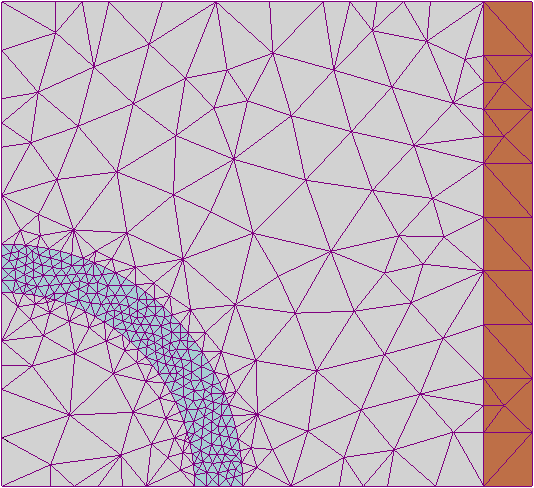
\includegraphics[width=0.25\textwidth]{unstructured_mesh}
    \caption{Unstructured grid in 2D}
    \label{fig:unstructured_mesh}

    \small Source: By I, Zureks, CC BY-SA 3.0, %
    https://commons.wikimedia.org/w/index.php?curid=2358783
\end{figure}

Therefore, if the problem at hand lends itself to being modelled with structured
meshes, a more efficient solution can be achieved if we take advantage of the
structure. However, not all problems are easily described in terms of structured
meshes, making it necessary to consider unstructured ones as well. In some
cases, it may also be useful to build hybrid meshes that contain structured and
unstructured parts, leveraging the efficiency of structured meshes where the
geometry of the problem allows it, while using an unstructured topology where it
is necessary.

\subsection{Challenges}
In the past decades, numerous parallel hardware architectures have emerged and
become available for scientific research. The programming models of these are
often inherently different. CPUs, GPUs and FPGAs have varying degrees and
underlying physical implementations of parallelism. As an example, modern CPUs
contain multiple cores, but in each core, they usually also have vectorisation
units for the \textit{Single instruction, multiple data (SIMD)} type of
parallelism. This variability implies that in order to make full use of all of
their features and characteristics, these architectures need to be programmed in
potentially very different ways.

Another difficulty that has become relevant comparatively recently is the use of
hierarchical cache architectures. The need for those arises because the increase
in RAM speed has not generally been able to keep up with the pace of the
increase in processing speed. Therefore, more and more often the bottleneck in a
computation is not caused by the processing time but by waiting for data I/O.

Hierarchical cache architectures consist of multiple layers of memory storage
units organised such that higher-speed storage elements, which are often also
located closer to the processing unit, have lower storage capacity than
lower-speed elements. Main memory itself could be regarded as the last layer of
this hierarchy (if we do not consider hard disk drives or solid state drives),
having the highest storage capacity and the lowest speed. Efficient usage of the
cache hierarchy is vital in many applications, as accessing data from main
memory or from a slower cache level is potentially orders of magnitude slower
than accessing data in a high-speed cache unit. On many architectures,
manufacturers employ complex intelligent algorithms implemented within the
hardware that facilitate optimal cache usage, but still, writing software in a
cache-friendly way often has enormous impact on performance --- indeed,
cache-friendly programming often essentially means writing software in a way
that presents data to the processor such that its hardware cache algorithms can
be as efficient as possible. Most of the time it means that data regions that
are accessed close in time should be located close in memory. This is because
when the processor reads from memory, it always reads a fixed amount of data
even if it is more than what is immediately required. If the remaining data is
the same as is needed by the next computation cycle, it makes it unnecessary to
perform another (potentially very expensive) load operation from memory.

Scientific computations are often run on different parallel hardware devices to
speed up the simulations and make scientific experimentation faster. However,
programmers and scientists face a great challenge if they, because of the
differences in programming models and memory characteristics, have to maintain
separate code bases for each architecture. To write efficient code for these
devices, deep low-level knowledge of them is necessary and the scientists who
need to use them are usually not experts on any of these architectures and
definitely not several of them. Furthermore, maintenance of the code also
becomes more difficult, as any change introduced has to be applied to multiple
parts of the code base.

\subsection{Goals}

The goal of my thesis research is to design and implement an abstract interface
using which the scientific computations on spatial meshes can be expressed
easily, at a high level, without having to consider or even know about the
characteristics of the hardware they are to run on or the data structures that
should be used to make the computations efficient. The abstraction is designed
in such a way that it is possible to automatically generate efficient,
high-performance code for multiple hardware architectures from the code written
using the abstraction.

The separation of the scientific code from the parallelisation and data
structure code provides a solution to the problem of scientists not being
computer experts as well as making it unnecessary to write code by hand for
different hardware architectures and maintaining all the versions. At the same
time, the use of code generation, together with the careful design of the
abstraction, makes it possible to run the computations with high performance.

The abstraction also frees the user from having to interact directly with the
data structures used in the computations. One of its main advantages is that the
data structures behind the interface can be replaced, which is important, as
different data structures may be optimal for different computations.

A critical extension to the model that is present in our abstraction in contrast
to existing frameworks is allowing multiple materials to be present at the same
grid point. This allows for more complex simulations and including this new
feature is the primary motivation behind this thesis research project.

\section{Active libraries and DSLs}
\label{eDSLs}

% TODO
- DSLs (maybe from the OPS article also)?
- active library

\section{Existing solutions}

There are multiple frameworks that address the same or similar computation
models and challenges to the ones presented in this thesis. In this section, we
present two such frameworks: OPS \cite{OPS}, which can be used for computations
on structured meshes, and OP2 \cite{OP2}, which handles unstructured meshes.

\subsection{OPS}

% Introduction

The OPS (Oxford Parallel Library for Structured Mesh Solvers) Domain Specific
Active Library is a framework for parallel multi-block structured mesh
applications. Its goal is to provide a high-level abstraction for structured
mesh computations running on different parallel hardware architectures. The
motivation behind the framework can be summarised as follows:

\begin{itemize}
  \item separation of the domain specific, scientific code from the low-level
    implementation details such as data structures and explicit management of
    parallelism, thereby making it easier to use the framework
  \item providing a common interface for various hardware architectures
  \item extensibility and future proofing --- if a new hardware architecture
    appears, the framework can be extended to support it, and there is no need
    to modify the science code using the abstraction.
\end{itemize}

The framework achieves its goals by using an eDSL embedded in C/C++ and
generating efficient, optimised code for the desired platforms. For more
information on eDSLs, see \autoref{eDSLs}.

\subsubsection{API}

The OPS API consists of four components:

\begin{itemize}
  \item Blocks: a collection of structured grid blocks with dimensionality
    defined but with no size.
  \item Datasets: data defined on blocks, with size.
  \item Halos: a structure describing the connections between datasets defined
    on different blocks.
  \item Computations: description of a calculation on the grid, accessing
    datasets.
\end{itemize}

In order for OPS to be able to generate correct and efficient parallelised code,
two things are of great importance. The first is the assumption that the order
in which the elemental operations are performed on the grid points does not
change the overall result within machine precision. This is what allows OPS to
parallelise the computations. The second is that the data, once fed into OPS, is
owned by OPS and can only be accessed through opaque handlers. This makes it
possible for the framework to apply transformations to the data, which may
further help parallelisation and efficiency as different data structures may be
appropriate for different kinds of architectures and computations.

\subsubsection{Code generation}

In OPS, there are two fundamental techniques, the combination of which is used
to produce the parallelised and optimised implementation of the
computations. The first is \textit{code generation}, which provides the part of
the implementation that is specific to the target hardware architecture and
programming language. The second is \textit{back-end logic}, which contains the
parts of the implementation that are the same for all targets, for example data
movement among other things.

Although a single threaded, conventional header file implementation is
available, which can be compiled with a normal C/C++ compiler, the main use case
of OPS is using actual code generation for the target platform and
language. This makes it possible to generate specific code for the platform and
give the target language's compiler the largest possible amount of information,
also taking into account the characteristics of the computation at hand. The
target compiler can then make use of the information by optimising the resulting
machine code. Targets for OPS include single threaded applications as well as
parallelised ones using OpenMP, OpenACC, CUDA and OpenCL.

\subsubsection{Back-end logic}

\textit{Back-end logic} is the collection of algorithms that are not
hardware-specific, but common to all targets and handle the computations at a
higher level. Examples of these include data management, distributed memory
parallelism, data structure transformations, resilience and lazy execution
patterns. In the following paragraphs, we give a brief presentation of some of
these.

OPS supports \textit{distributed memory parallelism} by automatically
distributing individual blocks (or a collection of blocks) across multiple MPI
processes. The partitioning of the data is decided upon on the basis of the
iteration ranges on the blocks and the access patterns (stencils). The goal is
to minimise the necessary communication between the MPI processes and balance
the load evenly.  Data dependencies across partitions are satisfied using
\textit{ghost cells} and automatic intra-block halo exchanges. Data from other
partitions is sent in messages automatically on demand, the user does not have
to request it explicitly. To keep the data consistent across the MPI processes,
dirty bits are used.

Unforeseen crashes, often due to hardware failure or power outage, can never be
completely ruled out. Therefore, in long-running simulations, where restarting
the simulation from the beginning in case of a crash is infeasible, it becomes
important to backup the intermediary results during the computation. This
resilience is provided by the \textit{checkpointing and recovery} mechanism of
OPS, which saves the whole state space to disk periodically. Deciding the
checkpoints in the computation, where the backups are performed, is a
non-trivial task. Saving the whole state space to disk is an expensive process
in terms of performance, therefore it should not be done too often, and
preferably at times when the state space is small. Also, saving a dataset just
before it is overwritten in a subsequent computation is wasteful. In case of a
crash, the state space can be recovered from the backup. The computation
fast-forwards to the checkpoint and resumes progress from there.

\textit{Lazy execution} is another technique with which OPS seeks to improve its
performance. It exploits the fact that the intermediary results in a sequence of
computations (parallel loops) do not necessarily need to be computed at the
point where they appear in the source code, and their evaluation can be delayed
until the user actually accesses them, usually after a parallel loop involving
reduction. At that time, all the computations in the sequence can be applied at
once to each grid point, thereby only iterating through the mesh once, saving
the cost of the remaining iterations. Lazy execution can also eliminate the
computation of intermediate results that are never actually used in later
computations.

\subsubsection{Optimisations}

Lazy execution, mostly through the fusion of sequences of parallel loops,
enables further optimisations, some of which are described in this section.

OPS uses on-demand MPI messaging, which means that data is only sent to other
MPI processes when it is needed. However, message latency can become a
bottleneck in many applications, therefore different optimisation strategies can
be used to mitigate the problem. In many cases, the analysis of a sequence of
parallel loops made available by lazy execution makes it possible to aggregate
messages and send them at the same time, thereby reducing latency. Another
strategy is to run an unrelated computation in parallel with messaging, hiding
the latency of the latter. A third strategy useful in combination with the first
two is reordering parallel loops that do not have data dependencies on each
other in order to be able to better exploit the first two strategies.

These strategies help reduce latency, but the amount of data that needs to be
sent is not changed by them. Reduction in data exchange can be achieved by
various communication avoidance techniques, often involving redundant
computations and eliminating the evaluation of intermediary results that are not
needed later in the process.

A form of communication avoidance, \textit{cache blocking} or \textit{tiling}
aims to minimise data exchange between main memory and the cache. Accessing data
in main memory can be significantly more expensive than accessing data in cache,
and if data often needs to be moved into and out of the cache, it can have a
huge impact on the performance of the application. Executing a sequence of
parallel loops on the same dataset, if applied as it written in the source code,
executing an entire loop over the whole dataset before moving on to the next
one, may result in repeatedly evicting the cache and moving in new data if the
dataset does not fit in the cache. \textit{Tiling} avoids it by partitioning the
dataset into smaller blocks or tiles and executing the whole sequence of
parallel loops on one block at a time. This way, the same data can be reused and
read from cache every time a parallel loop is run on the block. As OPS uses lazy
execution and has a large amount of run-time information available such as
iteration ranges and access patterns, discovering data dependencies, and
consequently, partitioning the datasets into blocks, becomes much easier.

\subsection{OP2}

OP2 is an active library framework that essentially solves the same problems for
unstructured meshes as does OPS for structured meshes --- the solution of
partial differential equations (PDEs), computational electro-magnetics (CEM) and
computational fluid dynamics (CFD), among others. The means by which the two
frameworks operate are also the same as OP2, just like OPS, uses the concept of
Embedded Domain Specific Languages (eDSLs) to provide a way to generate
efficient parallelised code for different hardware architectures. The OP2 API
comes in two forms, both of which are eDSLs --- one of them is embedded in
C/C++, the other in Fortran.

\subsubsection{API}

The OP2 API consists of four main building blocks:

\begin{itemize}
  \item sets
  \item data on sets
  \item connectivity
  \item operations over sets
\end{itemize}

The elements of the most common types of sets are edges and (triangular or
quadrilateral) faces, though other types are also allowed. Data defined on sets
may include coordinates and edge weight among other things. As the mesh that the
set elements constitute parts of is unstructured, it is necessary to explicitly
define the connections between the elements of different sets --- which elements
of a set are adjacent to which elements of other sets. This is done by the
connectivity objects, which are also called mappings.

Operations over the sets are parallel loops that iterate over the elements of
one set, possibly accessing (reading, writing or both) the elements of other
sets through the mappings. If a loop accesses elements of other sets through the
mappings, it is called an indirect loop, otherwise it is referred to as a direct
loop.

The code written using the OP2 abstraction is analysed by the OP2
source-to-source compiler, which generates efficient parallelised source code
for the target platform. This can then be compiled with traditional compilers
and linked against the platform specific OP2 back-end. The design of the OP2
interface allows the source-to-source compiler to apply optimisations that rely
on information that would be very difficult or even impossible to infer had the
code been written in the form of normal, sequential loops.

As is the case with OPS, the OP2 framework also requires that the order in which
the operations are applied to the mesh elements should not affect the final
result within machine precision. This restriction is vital in order to allow OP2
to achieve the greatest possible amount of parallelism, thereby significantly
improving performance. Although this strategy comes at the price of giving up
bitwise reproducibility, in the vast majority of applications the gains in
performance far outweigh the negative effects, which, if needed, can be
mitigated by other means such as increasing the floating-point precision of the
calculations.

Another limitation of the framework is that OP2 does not support double
indirection along the mappings, i.e. starting from an element, accessing a
connecting element in another set through a mapping and then, from that element,
accessing yet another element through a different mapping of its own. In
addition, the mappings are static and cannot change once defined.

The targets supported by OP2 for code generation include single-threaded CPUs,
single SMP systems based on multi-core CPUs using OpenMP, single NVIDIA GPUs
using CUDA, clusters of CPUs using MPI and clusters of GPUs using MPI and CUDA.

\subsubsection{Parallelisation strategy}

In OP2, parallelisation is done on two levels. The first is distributed memory
parallelisation on a cluster containing several nodes, while the second is
parallelisation on a single node with shared memory architecture.

Parallelisation on the cluster level consists of partitioning the domain and
assigning every partition to a compute node. Import and export halos need to be
defined on the boundaries of the partitions to make data from other partitions
available to the compute nodes if they need it. As the size of these halos
determines the size of the MPI messages that need to be sent between the nodes,
the partitions should be chosen in such a way as to minimise the size of the
halos. In a distributed system, to an even greater extent than on a single node,
data movement (in the form of message passing) is often the most important
performance bottleneck, therefore the partitioning scheme plays a significant
role in making OP2 efficient.

Single-node parallelisation is dependent on the target hardware
architecture. CPUs provide multi-core shared-memory parallelism, and in addition
to that, vector units in each core. On GPUs, one can use multiple thread blocks,
each of which has multiple threads. Data movement between the main memory and
the CPU cores, or the main graphics memory and the GPU cores is very expensive
in terms of performance, thus the amount of data movement should be reduced as
much as possible, and OP2 uses various techniques to achieve this.

On the cluster level, partitioning the domain can be a very expensive operation,
so it is usually only done once, and all stages of the computation are executed
with the same partitions. On the other hand, on the single-node level, dividing
the data between the individual CPU or GPU threads can be done for every stage
of the computation, because between the stages, data is always located in main
memory, and repartitioning does not necessitate additional data movement.

\subsubsection{Data dependencies}

Parallelisation brings with itself the possibility of race conditions, which
must be avoided by the proper handling of data dependencies. An example of this
is a parallel loop over edges in which two different edges attempt to increment
the same cell (indirectly accessed through a mapping) at the same time. The two
levels of parallelisation, distributed memory parallelisation and shared memory
parallelisation, call for different solutions to the problem of data
dependencies.

On the level of distributed memory parallelisation, each set element (cell or
edge) belongs to a partition owned by an MPI process. Data dependencies between
different partitions are handled using the ``owner compute'' model, in which
each MPI process only updates the elements that are in its own partition. In the
case of an edge updating two cells in two different partitions, the edge
calculation is performed in both MPI processes. This introduces redundant
computations, but if the partitions are large enough, the proportion of
redundant computations becomes sufficiently small to be acceptable.

When a computation on a set element needs to access data from a neighbouring
partition, MPI message passing is used to provide the data. The set elements can
be divided into two categories: core elements do not need data from any other
partition and can be computed without message passing, while elements in halos
require that. This makes it possible to carry out the computations on the core
elements in parallel to performing the MPI messaging concerning the halo
elements. Halo elements can be further divided into elements on which redundant
computations will be performed and elements that will only be read by
computations in another partition.

On the level of a single node, the ``owner compute'' model would be inefficient
as the proportion of redundant computations would be significantly higher,
presenting an unacceptable overhead. For example, on the GPU, mini-partitions (a
part of the mesh that is handled by a single thread block) are too small and
their halos would be two large, resulting in an increased number of redundant
calculations. The same problem arises within a mini-partition when two threads
attempt to update the same element simultaniously. OP2's solution is the
``colouring'' approach in which each mini-partition (or each edge within a
single mini-partition) is assigned a colour such that no two mini-partitions or
edges of the same colour modify the same cell. This way, computations on
mini-partitions and edges of the same colour can be performed in parallel. The
colouring approach can also be used on multi-core CPUs with some modifications.

\subsection{Evaluation}

The two existing solutions presented above share most of their characteristics
with each other, and also with the abstraction presented in this thesis. Their
goal is to separate the scientific code from the implementation of parallelism
and data structures, provide a common interface for different hardware
architectures and make it easy to integrate new ones in the future. The
solutions they use to achieve their goals are also essentially the same. Both of
them employ one or more Embedded Domain Specific Languages (eDSLs) to provide an
interface that looks familiar to programmers of their respective host languages,
but use code generation to implement the highly specialised back-end logic that
ensures that the resulting code can utilise the full potential of the hardware
it is run on. Their differences lie in the class of problems they can be used to
solve, namely OPS can handle structured meshes while OP2 works on unstructured
meshes.

Our abstraction differs from OPS and OP2 in that it allows defining a varying
number of values on each grid point, independent of the other grid points. This
introduces some new challenges that are not present in the case of OPS and OP2,
as will be discussed later in this thesis. Currently the abstraction only
supports structured meshes, but we are planning to extend it to include
unstructured meshes as well. Our abstraction aims to provide a high-level eDSL
interface embedded in modern C++ that allows the user to be productive using the
framework, while at the same time providing enough information to the code
generation unit so that it can generate efficient and optimised code.

\chapter{Methods}

- data structures, compression

\chapter{Presentation of the work}

\section{The abstraction}
\section{C++ implementation}
\section{Algorithms}
\section{Measurements?}

\chapter{Future work}

Codegen, CUDA, advection

\chapter{Conclusion}

\printbibliography
\appendix
\chapter{List of appendices}

\end{document}
